\section{Project}

\subsection{Overview}

In figure~\ref{fig:overview} we identify the planned architecture of our product, including
its physical and software parts and their interaction with each other.

\begin{figure}
    \centering
    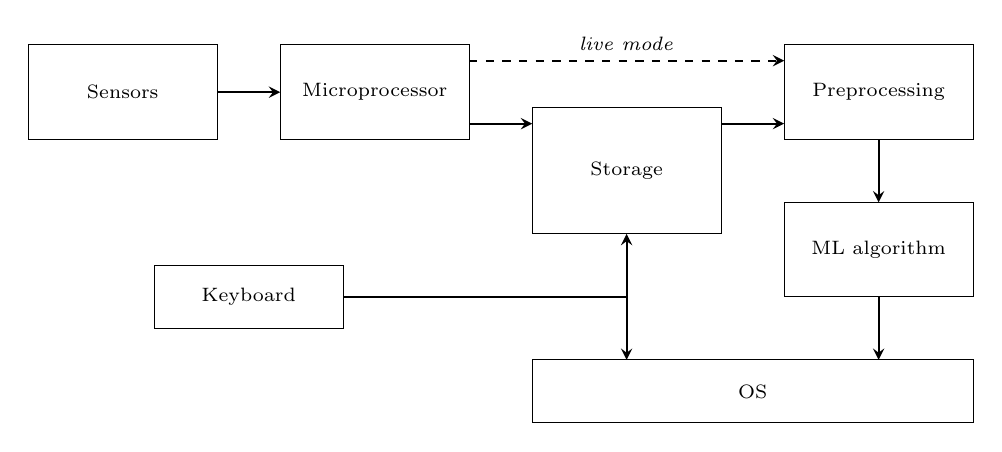
\begin{tikzpicture}[every node/.style={font=\scriptsize},scale=0.8]
        \tikzstyle{arrow} = [thick,->,>=stealth]
        \draw (0,0) rectangle (3,1.5) node[pos=.5] {Sensors};
        \draw (4,0) rectangle (7,1.5) node[pos=.5] {Microprocessor};
        \draw (2,-2) rectangle (5,-3) node[pos=.5] {Keyboard};
        \draw (8,0.5) rectangle (11,-1.5) node[pos=.5] {Storage};
        \draw (12,0) rectangle (15,1.5) node[pos=.5] {Preprocessing};
        \draw (12,-1) rectangle (15,-2.5) node[pos=.5] {ML algorithm};
        \draw (8,-3.5) rectangle (15,-4.5) node[pos=.5] {OS};

        \draw [arrow] (3, 0.75) -- (4, 0.75);
        \draw [arrow] (7, 0.25) -- (8, 0.25);
        \draw [arrow] (11, 0.25) -- (12, 0.25);
        \draw [arrow] (13.5, 0) -- (13.5, -1);
        \draw [arrow] (13.5, -2.5) -- (13.5, -3.5);
        \draw [arrow] (5, -2.5) -| (9.5, -1.5);
        \draw [arrow] (5, -2.5) -| (9.5, -3.5);
        \draw [dashed, arrow] (7, 1.25) -- node[anchor=south]{\textit{live mode}}(12, 1.25);
    \end{tikzpicture}
    \caption{Project overview}
    \label{fig:overview}
\end{figure}


For planning, building and connecting the hardware device, we will seek
assistance from the group Technical Aspects of Multimodal Systems (TAMS) from the
Department of Informatics of the University of Hamburg.

For developing the major software parts (preprocessing and machine learning) we
are looking forward to a  cooperation with the group Knowledge Technology
(WTM), also from the Department of Informatics of the University of Hamburg.

\subsection{Scope}

We shall now express the foreseeable scope of the project:

For the hardware device we first have to research suitable components and order
these. We have listed an estimation of the required hardware components including
their prices in Table~\ref{tbl:pricesheet}.

\begin{table}[htb]
    \centering
    \begin{tabu}{lrrr}
        \tabucline[1pt]{-} 
        \textbf{Component} & \textbf{EUR/unit} & \textbf{Count} & \textbf{Total/EUR} \\
        \tabucline[1pt]{-} 
        IMU & 10-20 & 12 & 120-240 \\
        Processor & 20-50 & 1-2 & 40-100 \\
        Other & TBD & TBD & 0-100 \\
        \tabucline[1pt]{-} 
        \textbf{Total} &  &  & 160-340 \\
        \tabucline[1pt]{-} 
    \end{tabu}
    \caption{Estimated hardware requirements and costs}
    \label{tbl:pricesheet}
\end{table}

For the hardware part we will also have to work out how to actually connect the
sensors to the processor(s), retrieve data from the sensors, and transmit them
to the computer. We will also have to actually build the device and find a way
to attach the hardware to the hand without impeding hand movements too much.

For the software part, we will have to build some scaffolding to pass around
data between our different software components and into the operating system.
We need to write the recording software for generating learning and testing
datasets, and the preprocessing code. We will probably find some configurable
implementation of a suitable machine learning algorithm (which we have to
choose first), so we do not plan to implement that part ourselves.

We expect that the hardest problem to solve will be defining and implementing
the preprocessing steps as well as choosing and configuring the machine
learning algorithm.

Our main intent is to define suitable preprocessing methods for the task at
hand.  We do not expect to get fancy with the machine learning part initially,
instead we aim to use something simple and fast for the proof of concept. We
are considering neural networks, specifically simple recurrent networks, to be
suitable for this task. However, evaluation of this assumption shall be part of
our works.

Of course all our attempts need to be evaluated, so we also have to define
performance metrics and evaluate our system against these. Since we're able to
learn offline with recorded data, it will be possible to repeat experiments
with different parameters to find good configurations.

In figure~\ref{fig:toc} we outline our preliminary table of contents. 

